\documentclass[tikz]{standalone}

\usepackage{amsmath}
\usepackage{unicode-math}
\usepackage{mathtools}
\usepackage{derivative}

\setmainfont{Stix Two Text}
\setmathfont{Stix Two Math}

\usetikzlibrary{arrows.meta,fit,positioning}

\renewcommand{\familydefault}{\sfdefault}

% prefix equation numbers with section number
\numberwithin{equation}{section}

\DeclarePairedDelimiter{\ceil}{\lceil}{\rceil}
\DeclarePairedDelimiter{\floor}{\lfloor}{\rfloor}
\DeclarePairedDelimiter{\abs}{\lvert}{\rvert}
\DeclarePairedDelimiter{\norm}{\lVert}{\rVert}
\DeclarePairedDelimiter{\bra}{\langle}{\rvert}
\DeclarePairedDelimiter{\ket}{\lvert}{\rangle}
\DeclarePairedDelimiter{\expval}{\langle}{\rangle}
\DeclarePairedDelimiter{\norder}{\mathcolon}{\mathcolon}
\DeclarePairedDelimiter{\anorder}{\typecolon}{\typecolon}
	
\newcommand{\laplace}{\mbfnabla^2}
\newcommand{\trans}{{\scriptscriptstyle\mathsf{T}}}

\newcommand{\vdot}{\cdot}
\newcommand{\vcross}{\vectimes}
\newcommand{\vb}[1]{\symbfup{#1}}
\newcommand{\vu}[1]{\hat{\vb{#1}}}
\newcommand*\dd[2][\relax]{\mathop{\ifx\relax#1\odif{#2}\else \odif[order={#1}]{#2}\fi\,}}

\newcommand{\vacuum}{\ket*{\vb{0}}}

\DeclareMathOperator{\trace}{Tr}
\DeclareMathOperator{\sinc}{sinc}

\AtBeginDocument{
	\let\Re\relax
	\let\Im\relax
	\DeclareMathOperator{\Re}{Re}
	\DeclareMathOperator{\Im}{Im}

	\renewcommand{\div}{\mathop{\mbfnabla\vdot}}
	\newcommand{\curl}{\mathop{\mbfnabla\vectimes}}
}

\DeclarePairedDelimiterX{\comm}[2]{[}{]}{#1,#2}

\DeclarePairedDelimiterX{\braket}[2]{\langle}{\rangle}{#1\delimsize\vert#2}
\DeclarePairedDelimiterX{\ketbra}[1]{\lvert}{\rvert}{#1\rangle\delimsize\langle#1}



\usetikzlibrary{arrows.meta}

\begin{document}
    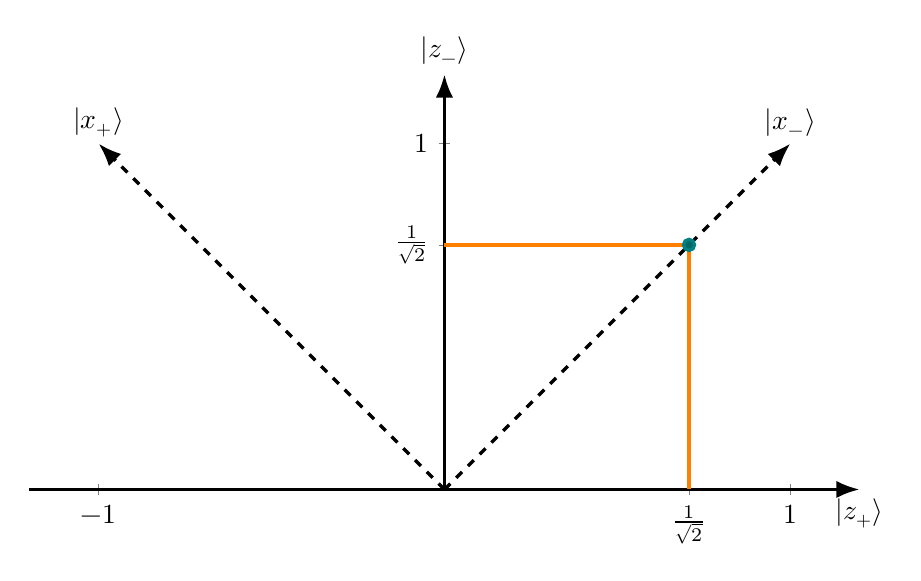
\begin{tikzpicture}
        \begin{axis}[
       		width=\linewidth,
            axis lines=center,
        	axis equal image,
            axis line style={very thick, -Latex},
            cycle list name=exotic,
            xmin=-1.2,
            xmax=+1.2,
            ymin=0,
            ymax=+1.2,
            xlabel={$\ket{z_+}$},
			xtick={-1,0.707,1},
			xticklabels={$-1$,$\frac{1}{\sqrt{2}}$,$1$},
			ytick={0.707,1},
			yticklabels={$\frac{1}{\sqrt{2}}$,$1$},
            ylabel={$\ket{z_-}$},
            x label style={anchor=north},
            y label style={anchor=south},
        ]
        	\draw[-Latex, very thick, dashed] (axis cs:0,0) -- (axis cs:1,1);
        	\draw[-Latex, very thick, dashed] (axis cs:0,0) -- (axis cs:-1,1);
        	\draw (axis cs:-1.0,1.06) node[]{$\ket{x_+}$};
        	\draw (axis cs:1.0,1.06) node[]{$\ket{x_-}$};
        	\addplot+[very thick] coordinates {(0.707,.707)};
        	\addplot+[very thick, no markers] coordinates {(0,.707) (.707,.707) (.707,0)};
        \end{axis}
    \end{tikzpicture}
\end{document}